\documentclass[twoside]{book}

% Packages required by doxygen
\usepackage{calc}
\usepackage{doxygen}
\usepackage{graphicx}
\usepackage[utf8]{inputenc}
\usepackage{makeidx}
\usepackage{multicol}
\usepackage{multirow}
\usepackage{textcomp}
\usepackage[table]{xcolor}

% Font selection
\usepackage[T1]{fontenc}
\usepackage{mathptmx}
\usepackage[scaled=.90]{helvet}
\usepackage{courier}
\usepackage{amssymb}
\usepackage{sectsty}
\renewcommand{\familydefault}{\sfdefault}
\allsectionsfont{%
  \fontseries{bc}\selectfont%
  \color{darkgray}%
}
\renewcommand{\DoxyLabelFont}{%
  \fontseries{bc}\selectfont%
  \color{darkgray}%
}

% Page & text layout
\usepackage{geometry}
\geometry{%
  a4paper,%
  top=2.5cm,%
  bottom=2.5cm,%
  left=2.5cm,%
  right=2.5cm%
}
\tolerance=750
\hfuzz=15pt
\hbadness=750
\setlength{\emergencystretch}{15pt}
\setlength{\parindent}{0cm}
\setlength{\parskip}{0.2cm}
\makeatletter
\renewcommand{\paragraph}{%
  \@startsection{paragraph}{4}{0ex}{-1.0ex}{1.0ex}{%
    \normalfont\normalsize\bfseries\SS@parafont%
  }%
}
\renewcommand{\subparagraph}{%
  \@startsection{subparagraph}{5}{0ex}{-1.0ex}{1.0ex}{%
    \normalfont\normalsize\bfseries\SS@subparafont%
  }%
}
\makeatother

% Headers & footers
\usepackage{fancyhdr}
\pagestyle{fancyplain}
\fancyhead[LE]{\fancyplain{}{\bfseries\thepage}}
\fancyhead[CE]{\fancyplain{}{}}
\fancyhead[RE]{\fancyplain{}{\bfseries\leftmark}}
\fancyhead[LO]{\fancyplain{}{\bfseries\rightmark}}
\fancyhead[CO]{\fancyplain{}{}}
\fancyhead[RO]{\fancyplain{}{\bfseries\thepage}}
\fancyfoot[LE]{\fancyplain{}{}}
\fancyfoot[CE]{\fancyplain{}{}}
\fancyfoot[RE]{\fancyplain{}{\bfseries\scriptsize Generated on Tue Apr 28 2015 10\-:05\-:01 for Zadanie21-\/04-\/2015 by Doxygen }}
\fancyfoot[LO]{\fancyplain{}{\bfseries\scriptsize Generated on Tue Apr 28 2015 10\-:05\-:01 for Zadanie21-\/04-\/2015 by Doxygen }}
\fancyfoot[CO]{\fancyplain{}{}}
\fancyfoot[RO]{\fancyplain{}{}}
\renewcommand{\footrulewidth}{0.4pt}
\renewcommand{\chaptermark}[1]{%
  \markboth{#1}{}%
}
\renewcommand{\sectionmark}[1]{%
  \markright{\thesection\ #1}%
}

% Indices & bibliography
\usepackage{natbib}
\usepackage[titles]{tocloft}
\setcounter{tocdepth}{3}
\setcounter{secnumdepth}{5}
\makeindex

% Hyperlinks (required, but should be loaded last)
\usepackage{ifpdf}
\ifpdf
  \usepackage[pdftex,pagebackref=true]{hyperref}
\else
  \usepackage[ps2pdf,pagebackref=true]{hyperref}
\fi
\hypersetup{%
  colorlinks=true,%
  linkcolor=blue,%
  citecolor=blue,%
  unicode%
}

% Custom commands
\newcommand{\clearemptydoublepage}{%
  \newpage{\pagestyle{empty}\cleardoublepage}%
}


%===== C O N T E N T S =====

\begin{document}

% Titlepage & ToC
\hypersetup{pageanchor=false}
\pagenumbering{roman}
\begin{titlepage}
\vspace*{7cm}
\begin{center}%
{\Large Zadanie21-\/04-\/2015 }\\
\vspace*{1cm}
{\large Generated by Doxygen 1.8.6}\\
\vspace*{0.5cm}
{\small Tue Apr 28 2015 10:05:01}\\
\end{center}
\end{titlepage}
\clearemptydoublepage
\tableofcontents
\clearemptydoublepage
\pagenumbering{arabic}
\hypersetup{pageanchor=true}

%--- Begin generated contents ---
\chapter{Hierarchical Index}
\section{Class Hierarchy}
This inheritance list is sorted roughly, but not completely, alphabetically\-:\begin{DoxyCompactList}
\item \contentsline{section}{Cook}{\pageref{class_cook}}{}
\item \contentsline{section}{Pizza}{\pageref{class_pizza}}{}
\item \contentsline{section}{Pizza\-Builder}{\pageref{class_pizza_builder}}{}
\begin{DoxyCompactList}
\item \contentsline{section}{Hawaiian\-Pizza\-Builder}{\pageref{class_hawaiian_pizza_builder}}{}
\item \contentsline{section}{Spicy\-Pizza\-Builder}{\pageref{class_spicy_pizza_builder}}{}
\end{DoxyCompactList}
\end{DoxyCompactList}

\chapter{Class Index}
\section{Class List}
Here are the classes, structs, unions and interfaces with brief descriptions\-:\begin{DoxyCompactList}
\item\contentsline{section}{\hyperlink{class_cook}{Cook} }{\pageref{class_cook}}{}
\item\contentsline{section}{\hyperlink{class_hawaiian_pizza_builder}{Hawaiian\-Pizza\-Builder} }{\pageref{class_hawaiian_pizza_builder}}{}
\item\contentsline{section}{\hyperlink{class_pizza}{Pizza} \\*Uzycie klasy }{\pageref{class_pizza}}{}
\item\contentsline{section}{\hyperlink{class_pizza_builder}{Pizza\-Builder} }{\pageref{class_pizza_builder}}{}
\item\contentsline{section}{\hyperlink{class_spicy_pizza_builder}{Spicy\-Pizza\-Builder} }{\pageref{class_spicy_pizza_builder}}{}
\end{DoxyCompactList}

\chapter{File Index}
\section{File List}
Here is a list of all files with brief descriptions\-:\begin{DoxyCompactList}
\item\contentsline{section}{include/\hyperlink{_dodaj_8h}{Dodaj.\-h} }{\pageref{_dodaj_8h}}{}
\item\contentsline{section}{src/\hyperlink{main_8cpp}{main.\-cpp} }{\pageref{main_8cpp}}{}
\item\contentsline{section}{src/\hyperlink{moj__pier_8cpp}{moj\-\_\-pier.\-cpp} }{\pageref{moj__pier_8cpp}}{}
\item\contentsline{section}{src/\hyperlink{silnia_8cpp}{silnia.\-cpp} }{\pageref{silnia_8cpp}}{}
\end{DoxyCompactList}

\chapter{Class Documentation}
\hypertarget{class_cook}{\section{Cook Class Reference}
\label{class_cook}\index{Cook@{Cook}}
}


{\ttfamily \#include $<$Dodaj.\-h$>$}

\subsection*{Public Member Functions}
\begin{DoxyCompactItemize}
\item 
void \hyperlink{class_cook_a57fcfa5be4b939f32d71f33c7dd4f0d8}{set\-Pizza\-Builder} (\hyperlink{class_pizza_builder}{Pizza\-Builder} $\ast$pb)
\item 
\hyperlink{class_pizza}{Pizza} $\ast$ \hyperlink{class_cook_aa6432a14102bd7abe71e5caad7d78f02}{get\-Pizza} ()
\item 
void \hyperlink{class_cook_a3c69ec4743390aacf285bd7a34e40b41}{construct\-Pizza} ()
\end{DoxyCompactItemize}


\subsection{Detailed Description}


Definition at line 96 of file Dodaj.\-h.



\subsection{Member Function Documentation}
\hypertarget{class_cook_a3c69ec4743390aacf285bd7a34e40b41}{\index{Cook@{Cook}!construct\-Pizza@{construct\-Pizza}}
\index{construct\-Pizza@{construct\-Pizza}!Cook@{Cook}}
\subsubsection[{construct\-Pizza}]{\setlength{\rightskip}{0pt plus 5cm}void Cook\-::construct\-Pizza (
\begin{DoxyParamCaption}
{}
\end{DoxyParamCaption}
)\hspace{0.3cm}{\ttfamily [inline]}}}\label{class_cook_a3c69ec4743390aacf285bd7a34e40b41}


Definition at line 107 of file Dodaj.\-h.

\hypertarget{class_cook_aa6432a14102bd7abe71e5caad7d78f02}{\index{Cook@{Cook}!get\-Pizza@{get\-Pizza}}
\index{get\-Pizza@{get\-Pizza}!Cook@{Cook}}
\subsubsection[{get\-Pizza}]{\setlength{\rightskip}{0pt plus 5cm}{\bf Pizza}$\ast$ Cook\-::get\-Pizza (
\begin{DoxyParamCaption}
{}
\end{DoxyParamCaption}
)\hspace{0.3cm}{\ttfamily [inline]}}}\label{class_cook_aa6432a14102bd7abe71e5caad7d78f02}


Definition at line 103 of file Dodaj.\-h.

\hypertarget{class_cook_a57fcfa5be4b939f32d71f33c7dd4f0d8}{\index{Cook@{Cook}!set\-Pizza\-Builder@{set\-Pizza\-Builder}}
\index{set\-Pizza\-Builder@{set\-Pizza\-Builder}!Cook@{Cook}}
\subsubsection[{set\-Pizza\-Builder}]{\setlength{\rightskip}{0pt plus 5cm}void Cook\-::set\-Pizza\-Builder (
\begin{DoxyParamCaption}
\item[{{\bf Pizza\-Builder} $\ast$}]{pb}
\end{DoxyParamCaption}
)\hspace{0.3cm}{\ttfamily [inline]}}}\label{class_cook_a57fcfa5be4b939f32d71f33c7dd4f0d8}


Definition at line 99 of file Dodaj.\-h.



The documentation for this class was generated from the following file\-:\begin{DoxyCompactItemize}
\item 
include/\hyperlink{_dodaj_8h}{Dodaj.\-h}\end{DoxyCompactItemize}

\hypertarget{class_hawaiian_pizza_builder}{\section{Hawaiian\-Pizza\-Builder Class Reference}
\label{class_hawaiian_pizza_builder}\index{Hawaiian\-Pizza\-Builder@{Hawaiian\-Pizza\-Builder}}
}


{\ttfamily \#include $<$Dodaj.\-h$>$}

Inheritance diagram for Hawaiian\-Pizza\-Builder\-:\begin{figure}[H]
\begin{center}
\leavevmode
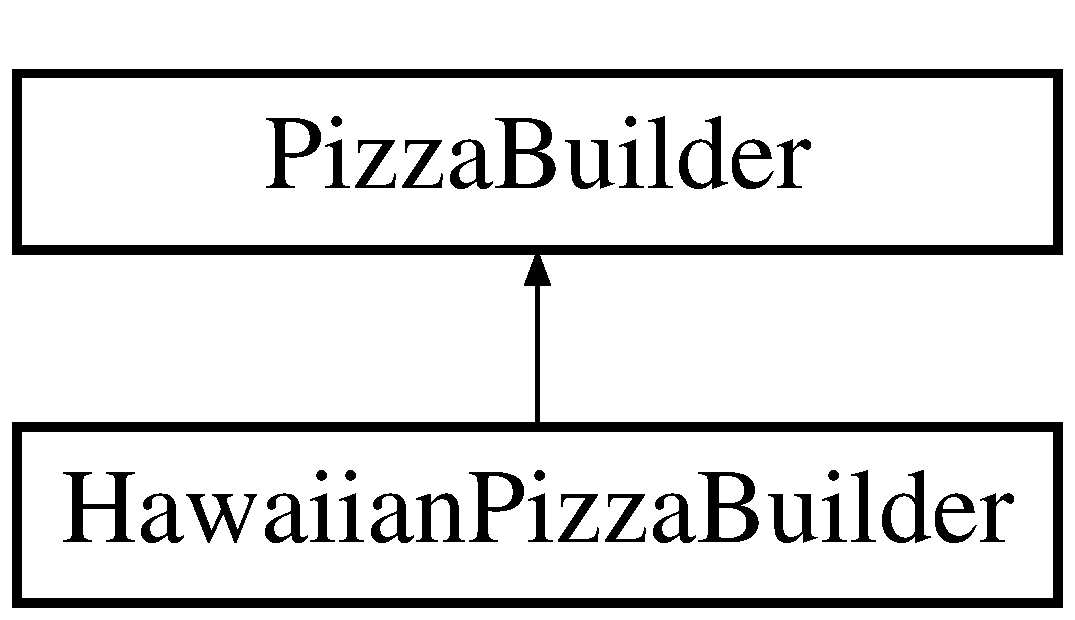
\includegraphics[height=2.000000cm]{class_hawaiian_pizza_builder}
\end{center}
\end{figure}
\subsection*{Public Member Functions}
\begin{DoxyCompactItemize}
\item 
virtual \hyperlink{class_hawaiian_pizza_builder_a621c6b7e508a206a5f85cea4e73fe747}{$\sim$\-Hawaiian\-Pizza\-Builder} ()
\item 
virtual void \hyperlink{class_hawaiian_pizza_builder_a0eddc6f115d76c24a9adfb86dc31a7cc}{build\-Dough} ()
\item 
virtual void \hyperlink{class_hawaiian_pizza_builder_abcfc366ad0ffcec8e93e19807b8eef18}{build\-Sauce} ()
\item 
virtual void \hyperlink{class_hawaiian_pizza_builder_af069af5d54a18d099a6ea6a4382fb42b}{build\-Topping} ()
\end{DoxyCompactItemize}
\subsection*{Additional Inherited Members}


\subsection{Detailed Description}


Definition at line 56 of file Dodaj.\-h.



\subsection{Constructor \& Destructor Documentation}
\hypertarget{class_hawaiian_pizza_builder_a621c6b7e508a206a5f85cea4e73fe747}{\index{Hawaiian\-Pizza\-Builder@{Hawaiian\-Pizza\-Builder}!$\sim$\-Hawaiian\-Pizza\-Builder@{$\sim$\-Hawaiian\-Pizza\-Builder}}
\index{$\sim$\-Hawaiian\-Pizza\-Builder@{$\sim$\-Hawaiian\-Pizza\-Builder}!HawaiianPizzaBuilder@{Hawaiian\-Pizza\-Builder}}
\subsubsection[{$\sim$\-Hawaiian\-Pizza\-Builder}]{\setlength{\rightskip}{0pt plus 5cm}virtual Hawaiian\-Pizza\-Builder\-::$\sim$\-Hawaiian\-Pizza\-Builder (
\begin{DoxyParamCaption}
{}
\end{DoxyParamCaption}
)\hspace{0.3cm}{\ttfamily [inline]}, {\ttfamily [virtual]}}}\label{class_hawaiian_pizza_builder_a621c6b7e508a206a5f85cea4e73fe747}


Definition at line 59 of file Dodaj.\-h.



\subsection{Member Function Documentation}
\hypertarget{class_hawaiian_pizza_builder_a0eddc6f115d76c24a9adfb86dc31a7cc}{\index{Hawaiian\-Pizza\-Builder@{Hawaiian\-Pizza\-Builder}!build\-Dough@{build\-Dough}}
\index{build\-Dough@{build\-Dough}!HawaiianPizzaBuilder@{Hawaiian\-Pizza\-Builder}}
\subsubsection[{build\-Dough}]{\setlength{\rightskip}{0pt plus 5cm}virtual void Hawaiian\-Pizza\-Builder\-::build\-Dough (
\begin{DoxyParamCaption}
{}
\end{DoxyParamCaption}
)\hspace{0.3cm}{\ttfamily [inline]}, {\ttfamily [virtual]}}}\label{class_hawaiian_pizza_builder_a0eddc6f115d76c24a9adfb86dc31a7cc}


Implements \hyperlink{class_pizza_builder_ab779fb4306ae03b3d82690f5939aaf22}{Pizza\-Builder}.



Definition at line 61 of file Dodaj.\-h.

\hypertarget{class_hawaiian_pizza_builder_abcfc366ad0ffcec8e93e19807b8eef18}{\index{Hawaiian\-Pizza\-Builder@{Hawaiian\-Pizza\-Builder}!build\-Sauce@{build\-Sauce}}
\index{build\-Sauce@{build\-Sauce}!HawaiianPizzaBuilder@{Hawaiian\-Pizza\-Builder}}
\subsubsection[{build\-Sauce}]{\setlength{\rightskip}{0pt plus 5cm}virtual void Hawaiian\-Pizza\-Builder\-::build\-Sauce (
\begin{DoxyParamCaption}
{}
\end{DoxyParamCaption}
)\hspace{0.3cm}{\ttfamily [inline]}, {\ttfamily [virtual]}}}\label{class_hawaiian_pizza_builder_abcfc366ad0ffcec8e93e19807b8eef18}


Implements \hyperlink{class_pizza_builder_a87b3cc72715e7775c8b36e610e8bb389}{Pizza\-Builder}.



Definition at line 65 of file Dodaj.\-h.

\hypertarget{class_hawaiian_pizza_builder_af069af5d54a18d099a6ea6a4382fb42b}{\index{Hawaiian\-Pizza\-Builder@{Hawaiian\-Pizza\-Builder}!build\-Topping@{build\-Topping}}
\index{build\-Topping@{build\-Topping}!HawaiianPizzaBuilder@{Hawaiian\-Pizza\-Builder}}
\subsubsection[{build\-Topping}]{\setlength{\rightskip}{0pt plus 5cm}virtual void Hawaiian\-Pizza\-Builder\-::build\-Topping (
\begin{DoxyParamCaption}
{}
\end{DoxyParamCaption}
)\hspace{0.3cm}{\ttfamily [inline]}, {\ttfamily [virtual]}}}\label{class_hawaiian_pizza_builder_af069af5d54a18d099a6ea6a4382fb42b}


Implements \hyperlink{class_pizza_builder_a46ff797a62789eca327a9ffab95b1b23}{Pizza\-Builder}.



Definition at line 69 of file Dodaj.\-h.



The documentation for this class was generated from the following file\-:\begin{DoxyCompactItemize}
\item 
include/\hyperlink{_dodaj_8h}{Dodaj.\-h}\end{DoxyCompactItemize}

\hypertarget{class_pizza}{\section{Pizza Class Reference}
\label{class_pizza}\index{Pizza@{Pizza}}
}


uzycie klasy  




{\ttfamily \#include $<$Dodaj.\-h$>$}

\subsection*{Public Member Functions}
\begin{DoxyCompactItemize}
\item 
void \hyperlink{class_pizza_a1a9bc97fa6c46d45d83134142773acb0}{set\-Dough} (const string \&dough)
\item 
void \hyperlink{class_pizza_ad9d05760ea59099ee00d44006d0622f3}{set\-Sauce} (const string \&sauce)
\item 
void \hyperlink{class_pizza_adc9f4d67313151e14ad380324d56d43e}{set\-Topping} (const string \&topping)
\item 
void \hyperlink{class_pizza_a7d812bc17133896f57459588988ffd47}{open} () const 
\end{DoxyCompactItemize}


\subsection{Detailed Description}
uzycie klasy 

Definition at line 7 of file Dodaj.\-h.



\subsection{Member Function Documentation}
\hypertarget{class_pizza_a7d812bc17133896f57459588988ffd47}{\index{Pizza@{Pizza}!open@{open}}
\index{open@{open}!Pizza@{Pizza}}
\subsubsection[{open}]{\setlength{\rightskip}{0pt plus 5cm}void Pizza\-::open (
\begin{DoxyParamCaption}
{}
\end{DoxyParamCaption}
) const\hspace{0.3cm}{\ttfamily [inline]}}}\label{class_pizza_a7d812bc17133896f57459588988ffd47}


Definition at line 22 of file Dodaj.\-h.

\hypertarget{class_pizza_a1a9bc97fa6c46d45d83134142773acb0}{\index{Pizza@{Pizza}!set\-Dough@{set\-Dough}}
\index{set\-Dough@{set\-Dough}!Pizza@{Pizza}}
\subsubsection[{set\-Dough}]{\setlength{\rightskip}{0pt plus 5cm}void Pizza\-::set\-Dough (
\begin{DoxyParamCaption}
\item[{const string \&}]{dough}
\end{DoxyParamCaption}
)\hspace{0.3cm}{\ttfamily [inline]}}}\label{class_pizza_a1a9bc97fa6c46d45d83134142773acb0}


Definition at line 10 of file Dodaj.\-h.

\hypertarget{class_pizza_ad9d05760ea59099ee00d44006d0622f3}{\index{Pizza@{Pizza}!set\-Sauce@{set\-Sauce}}
\index{set\-Sauce@{set\-Sauce}!Pizza@{Pizza}}
\subsubsection[{set\-Sauce}]{\setlength{\rightskip}{0pt plus 5cm}void Pizza\-::set\-Sauce (
\begin{DoxyParamCaption}
\item[{const string \&}]{sauce}
\end{DoxyParamCaption}
)\hspace{0.3cm}{\ttfamily [inline]}}}\label{class_pizza_ad9d05760ea59099ee00d44006d0622f3}


Definition at line 14 of file Dodaj.\-h.

\hypertarget{class_pizza_adc9f4d67313151e14ad380324d56d43e}{\index{Pizza@{Pizza}!set\-Topping@{set\-Topping}}
\index{set\-Topping@{set\-Topping}!Pizza@{Pizza}}
\subsubsection[{set\-Topping}]{\setlength{\rightskip}{0pt plus 5cm}void Pizza\-::set\-Topping (
\begin{DoxyParamCaption}
\item[{const string \&}]{topping}
\end{DoxyParamCaption}
)\hspace{0.3cm}{\ttfamily [inline]}}}\label{class_pizza_adc9f4d67313151e14ad380324d56d43e}


Definition at line 18 of file Dodaj.\-h.



The documentation for this class was generated from the following file\-:\begin{DoxyCompactItemize}
\item 
include/\hyperlink{_dodaj_8h}{Dodaj.\-h}\end{DoxyCompactItemize}

\hypertarget{class_pizza_builder}{\section{Pizza\-Builder Class Reference}
\label{class_pizza_builder}\index{Pizza\-Builder@{Pizza\-Builder}}
}


{\ttfamily \#include $<$Dodaj.\-h$>$}

Inheritance diagram for Pizza\-Builder\-:\begin{figure}[H]
\begin{center}
\leavevmode
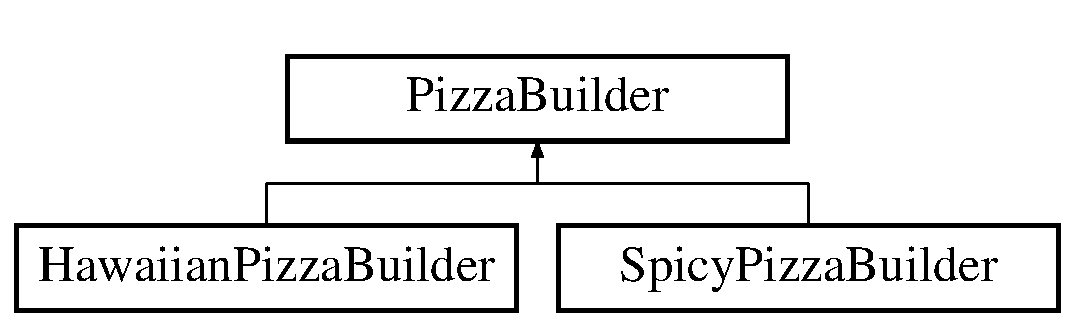
\includegraphics[height=2.000000cm]{class_pizza_builder}
\end{center}
\end{figure}
\subsection*{Public Member Functions}
\begin{DoxyCompactItemize}
\item 
virtual \hyperlink{class_pizza_builder_a424dc27395e06a4c38beca703c91c258}{$\sim$\-Pizza\-Builder} ()
\item 
\hyperlink{class_pizza}{Pizza} $\ast$ \hyperlink{class_pizza_builder_a95ce87757351da71ab03f400802a0d1a}{get\-Pizza} ()
\item 
void \hyperlink{class_pizza_builder_ad321d7aede0131b349c6853768ea1735}{create\-New\-Pizza\-Product} ()
\item 
virtual void \hyperlink{class_pizza_builder_ab779fb4306ae03b3d82690f5939aaf22}{build\-Dough} ()=0
\item 
virtual void \hyperlink{class_pizza_builder_a87b3cc72715e7775c8b36e610e8bb389}{build\-Sauce} ()=0
\item 
virtual void \hyperlink{class_pizza_builder_a46ff797a62789eca327a9ffab95b1b23}{build\-Topping} ()=0
\end{DoxyCompactItemize}
\subsection*{Protected Attributes}
\begin{DoxyCompactItemize}
\item 
\hyperlink{class_pizza}{Pizza} $\ast$ \hyperlink{class_pizza_builder_a095c1999e588b9db2d4fcec6e050e3a2}{m\-\_\-pizza}
\end{DoxyCompactItemize}


\subsection{Detailed Description}


Definition at line 34 of file Dodaj.\-h.



\subsection{Constructor \& Destructor Documentation}
\hypertarget{class_pizza_builder_a424dc27395e06a4c38beca703c91c258}{\index{Pizza\-Builder@{Pizza\-Builder}!$\sim$\-Pizza\-Builder@{$\sim$\-Pizza\-Builder}}
\index{$\sim$\-Pizza\-Builder@{$\sim$\-Pizza\-Builder}!PizzaBuilder@{Pizza\-Builder}}
\subsubsection[{$\sim$\-Pizza\-Builder}]{\setlength{\rightskip}{0pt plus 5cm}virtual Pizza\-Builder\-::$\sim$\-Pizza\-Builder (
\begin{DoxyParamCaption}
{}
\end{DoxyParamCaption}
)\hspace{0.3cm}{\ttfamily [inline]}, {\ttfamily [virtual]}}}\label{class_pizza_builder_a424dc27395e06a4c38beca703c91c258}


Definition at line 37 of file Dodaj.\-h.



\subsection{Member Function Documentation}
\hypertarget{class_pizza_builder_ab779fb4306ae03b3d82690f5939aaf22}{\index{Pizza\-Builder@{Pizza\-Builder}!build\-Dough@{build\-Dough}}
\index{build\-Dough@{build\-Dough}!PizzaBuilder@{Pizza\-Builder}}
\subsubsection[{build\-Dough}]{\setlength{\rightskip}{0pt plus 5cm}virtual void Pizza\-Builder\-::build\-Dough (
\begin{DoxyParamCaption}
{}
\end{DoxyParamCaption}
)\hspace{0.3cm}{\ttfamily [pure virtual]}}}\label{class_pizza_builder_ab779fb4306ae03b3d82690f5939aaf22}


Implemented in \hyperlink{class_spicy_pizza_builder_a31a9b83aff106bf255cdd7b07428cc8f}{Spicy\-Pizza\-Builder}, and \hyperlink{class_hawaiian_pizza_builder_a0eddc6f115d76c24a9adfb86dc31a7cc}{Hawaiian\-Pizza\-Builder}.

\hypertarget{class_pizza_builder_a87b3cc72715e7775c8b36e610e8bb389}{\index{Pizza\-Builder@{Pizza\-Builder}!build\-Sauce@{build\-Sauce}}
\index{build\-Sauce@{build\-Sauce}!PizzaBuilder@{Pizza\-Builder}}
\subsubsection[{build\-Sauce}]{\setlength{\rightskip}{0pt plus 5cm}virtual void Pizza\-Builder\-::build\-Sauce (
\begin{DoxyParamCaption}
{}
\end{DoxyParamCaption}
)\hspace{0.3cm}{\ttfamily [pure virtual]}}}\label{class_pizza_builder_a87b3cc72715e7775c8b36e610e8bb389}


Implemented in \hyperlink{class_spicy_pizza_builder_a74a4d62a67d118b8bbe94721847f38b4}{Spicy\-Pizza\-Builder}, and \hyperlink{class_hawaiian_pizza_builder_abcfc366ad0ffcec8e93e19807b8eef18}{Hawaiian\-Pizza\-Builder}.

\hypertarget{class_pizza_builder_a46ff797a62789eca327a9ffab95b1b23}{\index{Pizza\-Builder@{Pizza\-Builder}!build\-Topping@{build\-Topping}}
\index{build\-Topping@{build\-Topping}!PizzaBuilder@{Pizza\-Builder}}
\subsubsection[{build\-Topping}]{\setlength{\rightskip}{0pt plus 5cm}virtual void Pizza\-Builder\-::build\-Topping (
\begin{DoxyParamCaption}
{}
\end{DoxyParamCaption}
)\hspace{0.3cm}{\ttfamily [pure virtual]}}}\label{class_pizza_builder_a46ff797a62789eca327a9ffab95b1b23}


Implemented in \hyperlink{class_spicy_pizza_builder_a18fccc77e058f373deb851d61074df5b}{Spicy\-Pizza\-Builder}, and \hyperlink{class_hawaiian_pizza_builder_af069af5d54a18d099a6ea6a4382fb42b}{Hawaiian\-Pizza\-Builder}.

\hypertarget{class_pizza_builder_ad321d7aede0131b349c6853768ea1735}{\index{Pizza\-Builder@{Pizza\-Builder}!create\-New\-Pizza\-Product@{create\-New\-Pizza\-Product}}
\index{create\-New\-Pizza\-Product@{create\-New\-Pizza\-Product}!PizzaBuilder@{Pizza\-Builder}}
\subsubsection[{create\-New\-Pizza\-Product}]{\setlength{\rightskip}{0pt plus 5cm}void Pizza\-Builder\-::create\-New\-Pizza\-Product (
\begin{DoxyParamCaption}
{}
\end{DoxyParamCaption}
)\hspace{0.3cm}{\ttfamily [inline]}}}\label{class_pizza_builder_ad321d7aede0131b349c6853768ea1735}


Definition at line 43 of file Dodaj.\-h.

\hypertarget{class_pizza_builder_a95ce87757351da71ab03f400802a0d1a}{\index{Pizza\-Builder@{Pizza\-Builder}!get\-Pizza@{get\-Pizza}}
\index{get\-Pizza@{get\-Pizza}!PizzaBuilder@{Pizza\-Builder}}
\subsubsection[{get\-Pizza}]{\setlength{\rightskip}{0pt plus 5cm}{\bf Pizza}$\ast$ Pizza\-Builder\-::get\-Pizza (
\begin{DoxyParamCaption}
{}
\end{DoxyParamCaption}
)\hspace{0.3cm}{\ttfamily [inline]}}}\label{class_pizza_builder_a95ce87757351da71ab03f400802a0d1a}


Definition at line 39 of file Dodaj.\-h.



\subsection{Member Data Documentation}
\hypertarget{class_pizza_builder_a095c1999e588b9db2d4fcec6e050e3a2}{\index{Pizza\-Builder@{Pizza\-Builder}!m\-\_\-pizza@{m\-\_\-pizza}}
\index{m\-\_\-pizza@{m\-\_\-pizza}!PizzaBuilder@{Pizza\-Builder}}
\subsubsection[{m\-\_\-pizza}]{\setlength{\rightskip}{0pt plus 5cm}{\bf Pizza}$\ast$ Pizza\-Builder\-::m\-\_\-pizza\hspace{0.3cm}{\ttfamily [protected]}}}\label{class_pizza_builder_a095c1999e588b9db2d4fcec6e050e3a2}


Definition at line 51 of file Dodaj.\-h.



The documentation for this class was generated from the following file\-:\begin{DoxyCompactItemize}
\item 
include/\hyperlink{_dodaj_8h}{Dodaj.\-h}\end{DoxyCompactItemize}

\hypertarget{class_spicy_pizza_builder}{\section{Spicy\-Pizza\-Builder Class Reference}
\label{class_spicy_pizza_builder}\index{Spicy\-Pizza\-Builder@{Spicy\-Pizza\-Builder}}
}


{\ttfamily \#include $<$Dodaj.\-h$>$}

Inheritance diagram for Spicy\-Pizza\-Builder\-:\begin{figure}[H]
\begin{center}
\leavevmode
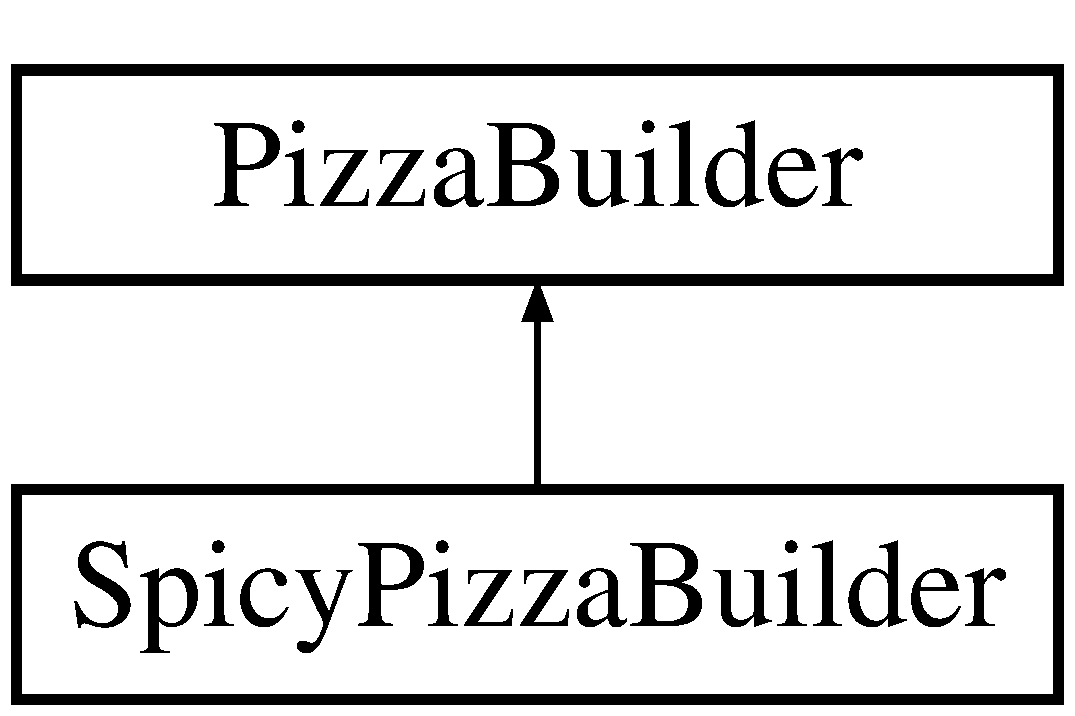
\includegraphics[height=2.000000cm]{class_spicy_pizza_builder}
\end{center}
\end{figure}
\subsection*{Public Member Functions}
\begin{DoxyCompactItemize}
\item 
virtual \hyperlink{class_spicy_pizza_builder_ada134c577c76bbe33589074d1eca989b}{$\sim$\-Spicy\-Pizza\-Builder} ()
\item 
virtual void \hyperlink{class_spicy_pizza_builder_a31a9b83aff106bf255cdd7b07428cc8f}{build\-Dough} ()
\item 
virtual void \hyperlink{class_spicy_pizza_builder_a74a4d62a67d118b8bbe94721847f38b4}{build\-Sauce} ()
\item 
virtual void \hyperlink{class_spicy_pizza_builder_a18fccc77e058f373deb851d61074df5b}{build\-Topping} ()
\end{DoxyCompactItemize}
\subsection*{Additional Inherited Members}


\subsection{Detailed Description}


Definition at line 75 of file Dodaj.\-h.



\subsection{Constructor \& Destructor Documentation}
\hypertarget{class_spicy_pizza_builder_ada134c577c76bbe33589074d1eca989b}{\index{Spicy\-Pizza\-Builder@{Spicy\-Pizza\-Builder}!$\sim$\-Spicy\-Pizza\-Builder@{$\sim$\-Spicy\-Pizza\-Builder}}
\index{$\sim$\-Spicy\-Pizza\-Builder@{$\sim$\-Spicy\-Pizza\-Builder}!SpicyPizzaBuilder@{Spicy\-Pizza\-Builder}}
\subsubsection[{$\sim$\-Spicy\-Pizza\-Builder}]{\setlength{\rightskip}{0pt plus 5cm}virtual Spicy\-Pizza\-Builder\-::$\sim$\-Spicy\-Pizza\-Builder (
\begin{DoxyParamCaption}
{}
\end{DoxyParamCaption}
)\hspace{0.3cm}{\ttfamily [inline]}, {\ttfamily [virtual]}}}\label{class_spicy_pizza_builder_ada134c577c76bbe33589074d1eca989b}


Definition at line 78 of file Dodaj.\-h.



\subsection{Member Function Documentation}
\hypertarget{class_spicy_pizza_builder_a31a9b83aff106bf255cdd7b07428cc8f}{\index{Spicy\-Pizza\-Builder@{Spicy\-Pizza\-Builder}!build\-Dough@{build\-Dough}}
\index{build\-Dough@{build\-Dough}!SpicyPizzaBuilder@{Spicy\-Pizza\-Builder}}
\subsubsection[{build\-Dough}]{\setlength{\rightskip}{0pt plus 5cm}virtual void Spicy\-Pizza\-Builder\-::build\-Dough (
\begin{DoxyParamCaption}
{}
\end{DoxyParamCaption}
)\hspace{0.3cm}{\ttfamily [inline]}, {\ttfamily [virtual]}}}\label{class_spicy_pizza_builder_a31a9b83aff106bf255cdd7b07428cc8f}


Implements \hyperlink{class_pizza_builder_ab779fb4306ae03b3d82690f5939aaf22}{Pizza\-Builder}.



Definition at line 80 of file Dodaj.\-h.

\hypertarget{class_spicy_pizza_builder_a74a4d62a67d118b8bbe94721847f38b4}{\index{Spicy\-Pizza\-Builder@{Spicy\-Pizza\-Builder}!build\-Sauce@{build\-Sauce}}
\index{build\-Sauce@{build\-Sauce}!SpicyPizzaBuilder@{Spicy\-Pizza\-Builder}}
\subsubsection[{build\-Sauce}]{\setlength{\rightskip}{0pt plus 5cm}virtual void Spicy\-Pizza\-Builder\-::build\-Sauce (
\begin{DoxyParamCaption}
{}
\end{DoxyParamCaption}
)\hspace{0.3cm}{\ttfamily [inline]}, {\ttfamily [virtual]}}}\label{class_spicy_pizza_builder_a74a4d62a67d118b8bbe94721847f38b4}


Implements \hyperlink{class_pizza_builder_a87b3cc72715e7775c8b36e610e8bb389}{Pizza\-Builder}.



Definition at line 84 of file Dodaj.\-h.

\hypertarget{class_spicy_pizza_builder_a18fccc77e058f373deb851d61074df5b}{\index{Spicy\-Pizza\-Builder@{Spicy\-Pizza\-Builder}!build\-Topping@{build\-Topping}}
\index{build\-Topping@{build\-Topping}!SpicyPizzaBuilder@{Spicy\-Pizza\-Builder}}
\subsubsection[{build\-Topping}]{\setlength{\rightskip}{0pt plus 5cm}virtual void Spicy\-Pizza\-Builder\-::build\-Topping (
\begin{DoxyParamCaption}
{}
\end{DoxyParamCaption}
)\hspace{0.3cm}{\ttfamily [inline]}, {\ttfamily [virtual]}}}\label{class_spicy_pizza_builder_a18fccc77e058f373deb851d61074df5b}


Implements \hyperlink{class_pizza_builder_a46ff797a62789eca327a9ffab95b1b23}{Pizza\-Builder}.



Definition at line 88 of file Dodaj.\-h.



The documentation for this class was generated from the following file\-:\begin{DoxyCompactItemize}
\item 
include/\hyperlink{_dodaj_8h}{Dodaj.\-h}\end{DoxyCompactItemize}

\chapter{File Documentation}
\hypertarget{_dodaj_8h}{\section{include/\-Dodaj.h File Reference}
\label{_dodaj_8h}\index{include/\-Dodaj.\-h@{include/\-Dodaj.\-h}}
}
\subsection*{Functions}
\begin{DoxyCompactItemize}
\item 
void \hyperlink{_dodaj_8h_a27a1864e1f4693766ae2596e6e205731}{hello} ()
\end{DoxyCompactItemize}
\subsection*{Variables}
\begin{DoxyCompactItemize}
\item 
float \hyperlink{_dodaj_8h_a1247f78c381ecedc869ac7da3f659494}{wynik} = liczby()
\end{DoxyCompactItemize}


\subsection{Function Documentation}
\hypertarget{_dodaj_8h_a27a1864e1f4693766ae2596e6e205731}{\index{Dodaj.\-h@{Dodaj.\-h}!hello@{hello}}
\index{hello@{hello}!Dodaj.h@{Dodaj.\-h}}
\subsubsection[{hello}]{\setlength{\rightskip}{0pt plus 5cm}void hello (
\begin{DoxyParamCaption}
{}
\end{DoxyParamCaption}
)}}\label{_dodaj_8h_a27a1864e1f4693766ae2596e6e205731}


Definition at line 6 of file moj\-\_\-pier.\-cpp.



\subsection{Variable Documentation}
\hypertarget{_dodaj_8h_a1247f78c381ecedc869ac7da3f659494}{\index{Dodaj.\-h@{Dodaj.\-h}!wynik@{wynik}}
\index{wynik@{wynik}!Dodaj.h@{Dodaj.\-h}}
\subsubsection[{wynik}]{\setlength{\rightskip}{0pt plus 5cm}wynik = liczby()}}\label{_dodaj_8h_a1247f78c381ecedc869ac7da3f659494}


Definition at line 2 of file Dodaj.\-h.


\hypertarget{dodawanie_8cpp}{\section{src/dodawanie.cpp File Reference}
\label{dodawanie_8cpp}\index{src/dodawanie.\-cpp@{src/dodawanie.\-cpp}}
}
{\ttfamily \#include \char`\"{}Dodaj.\-h\char`\"{}}\\*
\subsection*{Functions}
\begin{DoxyCompactItemize}
\item 
float \hyperlink{dodawanie_8cpp_a9cdd0e7e4a1a3de1d5211b630254c08a}{suma} (float a, float b)
\begin{DoxyCompactList}\small\item\em dodawanie dowolnych liczb \end{DoxyCompactList}\end{DoxyCompactItemize}


\subsection{Function Documentation}
\hypertarget{dodawanie_8cpp_a9cdd0e7e4a1a3de1d5211b630254c08a}{\index{dodawanie.\-cpp@{dodawanie.\-cpp}!suma@{suma}}
\index{suma@{suma}!dodawanie.cpp@{dodawanie.\-cpp}}
\subsubsection[{suma}]{\setlength{\rightskip}{0pt plus 5cm}float suma (
\begin{DoxyParamCaption}
\item[{float}]{a, }
\item[{float}]{b}
\end{DoxyParamCaption}
)}}\label{dodawanie_8cpp_a9cdd0e7e4a1a3de1d5211b630254c08a}


dodawanie dowolnych liczb 



Definition at line 4 of file dodawanie.\-cpp.


\hypertarget{main_8cpp}{\section{src/main.cpp File Reference}
\label{main_8cpp}\index{src/main.\-cpp@{src/main.\-cpp}}
}
{\ttfamily \#include $<$iostream$>$}\\*
{\ttfamily \#include \char`\"{}Dodaj.\-h\char`\"{}}\\*
\subsection*{Functions}
\begin{DoxyCompactItemize}
\item 
int \hyperlink{main_8cpp_ae66f6b31b5ad750f1fe042a706a4e3d4}{main} ()
\end{DoxyCompactItemize}


\subsection{Function Documentation}
\hypertarget{main_8cpp_ae66f6b31b5ad750f1fe042a706a4e3d4}{\index{main.\-cpp@{main.\-cpp}!main@{main}}
\index{main@{main}!main.cpp@{main.\-cpp}}
\subsubsection[{main}]{\setlength{\rightskip}{0pt plus 5cm}int main (
\begin{DoxyParamCaption}
{}
\end{DoxyParamCaption}
)}}\label{main_8cpp_ae66f6b31b5ad750f1fe042a706a4e3d4}


Definition at line 7 of file main.\-cpp.


\hypertarget{moj__pier_8cpp}{\section{src/moj\-\_\-pier.cpp File Reference}
\label{moj__pier_8cpp}\index{src/moj\-\_\-pier.\-cpp@{src/moj\-\_\-pier.\-cpp}}
}
{\ttfamily \#include $<$cstdio$>$}\\*
{\ttfamily \#include \char`\"{}Dodaj.\-h\char`\"{}}\\*
\subsection*{Functions}
\begin{DoxyCompactItemize}
\item 
void \hyperlink{moj__pier_8cpp_a27a1864e1f4693766ae2596e6e205731}{hello} ()
\end{DoxyCompactItemize}


\subsection{Function Documentation}
\hypertarget{moj__pier_8cpp_a27a1864e1f4693766ae2596e6e205731}{\index{moj\-\_\-pier.\-cpp@{moj\-\_\-pier.\-cpp}!hello@{hello}}
\index{hello@{hello}!moj_pier.cpp@{moj\-\_\-pier.\-cpp}}
\subsubsection[{hello}]{\setlength{\rightskip}{0pt plus 5cm}void hello (
\begin{DoxyParamCaption}
{}
\end{DoxyParamCaption}
)}}\label{moj__pier_8cpp_a27a1864e1f4693766ae2596e6e205731}


Definition at line 6 of file moj\-\_\-pier.\-cpp.


%--- End generated contents ---

% Index
\newpage
\phantomsection
\addcontentsline{toc}{chapter}{Index}
\printindex

\end{document}
